% Copyright 2004 by Till Tantau <tantau@users.sourceforge.net>.
%
% In principle, this file can be redistributed and/or modified under
% the terms of the GNU Public License, version 2.
%
% However, this file is supposed to be a template to be modified
% for your own needs. For this reason, if you use this file as a
% template and not specifically distribute it as part of a another
% package/program, I grant the extra permission to freely copy and
% modify this file as you see fit and even to delete this copyright
% notice. 

\documentclass[aspectratio=169]{beamer}
%\documentclass{beamer}

\setbeamersize{text margin left=10mm, text margin right=10mm}

\defbeamertemplate{headline}{my header}{%
\vskip1pt%
\makebox[0pt][l]{\,\insertshortauthor}%
\hspace*{\fill}\insertshorttitle/\insertshortsubtitle\hspace*{\fill}%
\llap{\insertpagenumber/\insertpresentationendpage\,}
}
\setbeamertemplate{headline}[my header]

\usepackage{graphicx}
\usepackage{soul}
\usepackage{tkz-euclide}
\usetikzlibrary{calc}
\usepackage[]{algorithm2e}
\usepackage{changepage}
\usepackage{amssymb}
\usepackage{xcolor}
\usepackage{mathtools}
\usepackage{tcolorbox}
\usepackage{tikz}
\usetikzlibrary{arrows}
\usepackage{tikz-3dplot}
\usepackage{tkz-euclide}
\usepackage{circuitikz}
\usepackage{pgfplots}
\pgfplotsset{width=7cm,compat=1.8}

\usetikzlibrary{positioning}
% \usepackage[math]{cellspace}
% \cellspacetoplimit 4pt
% \cellspacebottomlimit 4pt
%\usetikzlibrary{arrows.meta}
% sqare of half axes
\newcommand{\asa}{3}
\newcommand{\bsa}{1}
\newcommand{\csa}{0.25}
% view angle
\tdplotsetmaincoords{70}{135}

%\setbeamertemplate{itemize items}{-}

%\usepackage{helvet}
\usefonttheme{professionalfonts} % using non standard fonts for beamer
%\usefonttheme{serif} % default family is serif
%\usepackage{fontspec}
%\setmainfont{Liberation Serif}

% There are many different themes available for Beamer. A comprehensive
% list with examples is given here:
% http://deic.uab.es/~iblanes/beamer_gallery/index_by_theme.html
% You can uncomment the themes below if you would like to use a different
% one:
%\usetheme{AnnArbor}
%\usetheme{Antibes}
%\usetheme{Bergen}
%\usetheme{Berkeley}
%\usetheme{Berlin}
%\usetheme{Boadilla}
%\usetheme{boxes}
%\usetheme{CambridgeUS}
%\usetheme{Copenhagen}
%\usetheme{Darmstadt}
%\usetheme{default}
%\usetheme{Frankfurt}
%\usetheme{Goettingen}
%\usetheme{Hannover}
%\usetheme{Ilmenau}
%\usetheme{JuanLesPins}
%\usetheme{Luebeck}
%\usetheme{Madrid}
%\usetheme{Malmoe}
%\usetheme{Marburg}
%\usetheme{Montpellier}
%\usetheme{PaloAlto}
%\usetheme{Pittsburgh}
%\usetheme{Rochester}
%\usetheme{Singapore}
%\usetheme{Szeged}
%\usetheme{Warsaw}

\def\mf{\ensuremath\mathbf}
\def\mb{\ensuremath\mathbb}
\def\lp{\ensuremath\left(}
\def\rp{\ensuremath\right)}
\def\lv{\ensuremath\left\lvert}
\def\rv{\ensuremath\right\rvert}
\def\lV{\ensuremath\left\lVert}
\def\rV{\ensuremath\right\rVert}
\def\lc{\ensuremath\left\{}
\def\rc{\ensuremath\right\}}
\def\bmx{\ensuremath\begin{bmatrix*}[r]}
\def\emx{\ensuremath\end{bmatrix*}}
\def\bmxc{\ensuremath\begin{bmatrix*}[c]}


\newcommand{\demoex}[2]{\onslide<#1->\begin{color}{black!60} #2 \end{color}}
\newcommand{\anim}[3]{\onslide<#1->{\begin{color}{#2!60} #3 \end{color}}}



\title{Linear Systems}

% A subtitle is optional and this may be deleted
\subtitle{Singular Value Decomposition}

\author{Sivakumar Balasubramanian}
% - Give the names in the same order as the appear in the paper.
% - Use the \inst{?} command only if the authors have different
%   affiliation.

\institute[Christian Medical College] % (optional, but mostly needed)
{
  \inst{}%
  Department of Bioengineering\\
  Christian Medical College, Bagayam\\
  Vellore 632002
}
% - Use the \inst command only if there are several affiliations.
% - Keep it simple, no one is interested in your street address.

\date{}
% - Either use conference name or its abbreviation.
% - Not really informative to the audience, more for people (including
%   yourself) who are reading the slides online

\subject{Lecture notes on linear systems}
% This is only inserted into the PDF information catalog. Can be left
% out. 

% If you have a file called "university-logo-filename.xxx", where xxx
% is a graphic format that can be processed by latex or pdflatex,
% resp., then you can add a logo as follows:

% \pgfdeclareimage[height=0.5cm]{university-logo}{university-logo-filename}
% \logo{\pgfuseimage{university-logo}}

% Delete this, if you do not want the table of contents to pop up at
% the beginning of each subsection:
\AtBeginSubsection[]
{
  \begin{frame}<beamer>{Outline}
    \tableofcontents[currentsection,currentsubsection]
  \end{frame}
}

% Let's get started
\begin{document}

\pgfplotsset{
  compat=1.8,
  colormap={whitered}{color(0cm)=(white); color(1cm)=(orange!75!red)}
}


\begin{frame}
  \titlepage
\end{frame}

% \begin{frame}[t]{References}
% \begin{itemize}
%     \item G Strang, Linear Algebra: Chapters .
% \end{itemize} 
% \end{frame}


\begin{frame}[t]{Matrices are basis dependent}
\begin{itemize}
    \item Linear transformations represented as matrices depend on the choice of basis.

    For example, if $\mf{A}: \mb{R}^n \to \mb{R}^n$represents a linear transformation in the standard basis, then the same transformation in a basis $V$ is given by,
    \[ \mf{V}^{-1}\mf{A}\mf{V}: \text{Similarity transformation} \]

    \item In fact, for specific a choice of basis, it is possible to have the simplest possible representation for a linear transformation $\longrightarrow$ \textit{Eigen decomposition}.

    When a matrix $\mf{A}$ has $n$ eigenpairs $\lc\lp\lambda_i, \mf{x}_i\rp\rc_{i=1}^{n}$, with linearly independent eigenvectors, we have
    \[ \mf{A} = \mf{X}\mf{\Lambda}\mf{X}^{-1} \]

    \item What about rectangular matrices $\mf{A} \in \mb{R}^{n \times m}$? Can we talk about ``similar'' matrices in this case?
\end{itemize}
\end{frame}


\begin{frame}[t]{Matrix equivalence}
\begin{itemize}
    \item Consider a linear transformation $T:\mb{R}^{n} \to \mb{R}^m$, such that $\mf{y} = T\lp\mf{x}\rp$, where $\mf{x} \in \mb{R}^n$ and $\mf{y} \in \mb{R}^m$. $T$ can be represented as a matrix $\mf{A}$, such that $\mf{y} = \mf{A}\mf{x}$.

    \item Exact entries of $\mf{A}$ will depend on the choice of basis for both the input and the output spaces. Let us assume that the matrix $\mf{A}$ is the representation when the standard basis is used for the input and output spaces.

    \item If a different set of basis are chosen for the input and output spaces, namely $V = \lc\mf{v}_i\rc_{i=1}^{n}\,\,\lp\mf{v}_i \in \mb{R}^n\rp$ and $W = \lc\mf{w}_i\rc_{i=1}^{m}\,\,\lp\mf{w}_i \in \mb{R}^m\rp$. Then the corresponding matrix representation for the linear transformation $T$ is,
    \[ \mf{A}_{VW} = \mf{W}^{-1}\mf{A}\mf{V} \]
    where, the $\mf{V} = \bmx\mf{v}_1 & \mf{v}_2 & \ldots & \mf{v}_n\emx$ and $\mf{W} = \bmx\mf{w}_1 & \mf{w}_2 & \ldots & \mf{w}_m\emx$.

    \item $\mf{A}$ and $\mf{A}_{VW}$ are called \textit{equivalent matrices}.
\end{itemize}
\end{frame}


\begin{frame}[t]{Singular Value Decomposition: Diagonalizing any matrix}
\begin{itemize}
    \item Eigen-decomposition provided a way to do this for a square matrix with full rank. $\mf{A} = \mf{X}\mf{\Lambda}\mf{X}^{-1}$. When $\mf{A}$ is symmetric, $\mf{A} = \mf{Q}\mf{\Lambda}\mf{Q}^\top$.

    \item For rectangular and rank-deficient matrices, we can do this using \textit{singular value decomposition}.

    \item Consider a matrix $\mf{A} \in \mb{R}^{n \times m}$ with $rank\lp\mf{A}\rp = r$.
    \[ \mf{A} = \mf{U}\mf{\Sigma}\mf{V}^\top = \bmx \mf{u}_1 & \mf{u}_2 & \ldots & \mf{u}_m\emx
    \bmx \mf{D} & \mf{0}\\
    \mf{0} & \mf{0} \emx \bmx \mf{v}_1 & \mf{v}_2 & \ldots & \mf{v}_n \emx^\top\]
    where, $\mf{U} \in \mb{R}^{n \times n}$, $\mf{U}\mf{U}^\top = \mf{I}_n$; $\mf{V}\in \mb{R}^{m \times m}$, $\mf{V}\mf{V}^\top = \mf{I}_m$; and $\mf{D} = \mathrm{diag}\lp\sigma_1 \ldots \sigma_r\rp$.

    \item Columns $\mf{U}$ are eigenvectors of $\mf{A}^\top\mf{A}$, forming an orthonormal basis for $\mb{R}^m$.

    \item Columns $\mf{V}$ are eigenvectors of $\mf{A}\mf{A}^\top$, forming an orthonormal basis for $\mb{R}^n$.

    \item $\sigma_i^2 = \lambda_i$, where $\lambda_i$s are the eigenvalues of $\mf{A}^\top\mf{A}$ and $\mf{A}\mf{A}^\top$.
\end{itemize}
\end{frame}


\begin{frame}[t]{Singular Value Decomposition: Diagonalizing any matrix}
\begin{itemize}
    \item For $\mf{A}$,
    \vspace{-0.5cm}
    \[ C\lp\mf{A}\rp = span\lc\hat{\mf{u}}_{1} \ldots \hat{\mf{u}}_{r}\rc\,\,\,\,\, N\lp\mf{A}^\top\rp =  span\lc\hat{\mf{u}}_{r+1} \ldots \hat{\mf{u}}_{m}\rc \]\vspace{-0.8cm}
    \[ C\lp\mf{A}^\top\rp = span\lc\hat{\mf{v}}_{1} \ldots \hat{\mf{v}}_{r}\rc\,\,\,\,\, N\lp\mf{A}\rp = span\lc\hat{\mf{v}}_{r+1} \ldots \hat{\mf{v}}_{n}\rc \]\vspace{-0.2cm}

    where, the $\hat{\mf{u}}_i$s and the $\hat{\mf{v}}_i$s are any orthonormal basis for $\mb{R}^m$ and $\mb{R}^n$, respectively.
    \vspace{-0.2cm}
    {\small $$\hat{\mf{U}}_{cs} = \bmx\hat{\mf{u}}_{1} \ldots \hat{\mf{u}}_{r}\emx,\,\, \hat{\mf{U}}_{lns} = \bmx\hat{\mf{u}}_{r+1} \ldots \hat{\mf{u}}_{m}\emx,\,\, \hat{\mf{V}}_{rs} = \bmx\hat{\mf{v}}_{1} \ldots \hat{\mf{v}}_{r}\emx,\,\, \hat{\mf{V}}_{ns} = \bmx\hat{\mf{v}}_{r+1} \ldots \hat{\mf{v}}_{n}\emx$$}
    \vspace{-0.5cm}

    \item Now, $\mf{A}$ can be written as,
    \vspace{-0.3cm}
    \[ \mf{A} = \bmx\hat{\mf{U}}_{cs} & \hat{\mf{U}}_{lns}\emx \bmx \mf{R} & \mf{0}\\ \mf{0} & \mf{0} \emx \bmx\hat{\mf{V}}_{rs}^\top \\ \hat{\mf{V}}_{ns}^\top\emx \]\vspace{-0.4cm}

    where, $\mf{R} \in \mb{R}^{r \times r}$.

    It can be shown that two orthogonal matrices $\mf{P}$ and $\mf{Q}$ can be chosen, such that
    \[ \mf{A} = \bmx\hat{\mf{U}}_{cs} & \hat{\mf{U}}_{lns}\emx \mf{P} \bmx \mf{D} & \mf{0}\\ \mf{0} & \mf{0} \emx \mf{Q}^\top \bmx\hat{\mf{V}}_{rs}^\top \\ \hat{\mf{V}}_{ns}^\top\emx = \mf{U}\mf{\Sigma}\mf{V}^\top \]
\end{itemize}
\end{frame}


\begin{frame}[t]{Singular Value Decomposition: Diagonalizing any matrix}
\[ \mf{A} = \mf{U}\mf{\Sigma}\mf{V}^\top = \bmx \mf{u}_1 & \mf{u}_2 & \ldots & \mf{u}_m\emx \bmx \mf{D} & \mf{0}\\ \mf{0} & \mf{0} \emx \bmx \mf{v}_1 & \mf{v}_2 & \ldots \mf{v}_n \emx^\top\]

\begin{itemize}
    \item Orthonormal basis for $C\lp\mf{A}\rp \rightarrow \lc\mf{u}_{1}\ldots\mf{u}_{r}\rc$.
    
    \item Orthonormal basis for $N\lp\mf{A}^\top\rp \rightarrow \lc\mf{u}_{r+1}\ldots\mf{u}_{m}\rc$.
    
    \item Orthonormal basis for $C\lp\mf{A}^\top\rp \rightarrow \lc\mf{v}_{1}\ldots\mf{v}_{r}\rc$.
    \item Orthonormal basis for $N\lp\mf{A}\rp \rightarrow \lc\mf{v}_{r+1}\ldots\mf{v}_{n}\rc$.
    
    \item $\mf{D} = \bmxc \sigma_{1} & \ldots & 0\\\vdots & \ddots & \vdots\\0 & \ldots & \sigma_r\emx$, $\sigma_1 \geq \sigma_2 \geq \ldots \geq \sigma_r > 0$.

    \item Reduced SVD: $\mf{A} = \bmxc\mf{u}_1 \ldots \mf{u}_r\emx \bmxc \sigma_{1} & \ldots & 0\\\vdots & \ddots & \vdots\\0 & \ldots & \sigma_r\emx \bmxc\mf{v}_1^\top\\\vdots\\\mf{v}_r^\top\emx $
\end{itemize}
\end{frame}


\begin{frame}[t]{Singular Value Decomposition: Diagonalizing any matrix}
Find the SVD of $ \mf{A} = \bmx 1 & -1 \\ 1 & 1 \\ 0 & 1 \emx$.
\end{frame}


\begin{frame}[t]{Singular Value Decomposition: Diagonalizing any matrix}
Find the SVD of $ \mf{A} = \bmx 1 & -1 \\ 1 & -1 \\ 1 & -1 \emx$.
\end{frame}


% \begin{frame}[t]{Geometry of SVD}
% \begin{columns}
% \begin{column}{0.3\textwidth}
% \begin{scriptsize}
% $\mf{y} = \mf{Ax}$, where $\mf{A} = \mf{U}\mf{\Sigma}\mf{V}^\top$, $\mf{A} \in \mb{R}^{n \times n}$ and $rank\lp\mf{A}\rp = n$. \vspace{0.2cm}

% $1 = \lV\mf{x}\rV^2 = \lV\mf{A}^{-1}\mf{y}\rV^2$\vspace{0.1cm}

% $ = \mf{y}^\top\mf{A}^{-T}\mf{A}^{-1}\mf{y}$\vspace{0.1cm}

% $ = \mf{y}^\top\lp\mf{V}\mf{\Sigma}^{-1}\mf{U}^\top\rp^\top\mf{V}\mf{\Sigma}^{-1}\mf{U}^\top\mf{y}$\vspace{0.1cm}

% $ = \mf{y}^\top\mf{U}\mf{\Sigma}^{-1}\mf{V}^\top\mf{V}\mf{\Sigma}^{-1}\mf{U}^\top\mf{y}$\vspace{0.1cm}

% $ = \mf{w}^\top\mf{\Sigma}^{-2}\mf{w}$\vspace{0.1cm}

% where, $\mf{w} = \mf{U}^\top\mf{y}$; %and $\mf{\Sigma}^{-2} = \bmxc \mf{D}^{-2} & \mf{0}\\\mf{0} & \mf{0}\emx$.

% \[ x_1^2 + \ldots + x_n^2 = \frac{w_1^2}{\sigma_1^2} + \frac{w_2^2}{\sigma_2^2} + \ldots + \frac{w_n^2}{\sigma_n^2} = 1\]
% \end{scriptsize}
% \end{column}
% \begin{column}{0.7\textwidth}
% \begin{center}
%     \begin{tikzpicture}[scale=0.75]
%     \draw[gray, -latex, line width=0.1mm] (-2, 0) -- (2, 0) node[below] {$\mf{e}_1$};
%     \draw[gray, -latex, line width=0.1mm] (0, -1.5) -- (0, 1.5) node[above] {$\mf{e}_2$};
%     \draw[thick] (0,0) circle (1);
%     \draw[blue, -latex, line width=0.2mm] (0, 0) -- (1/1.414, 1/1.414) node[right] {$\mf{v}_1$};
%     \draw[blue, -latex, line width=0.2mm] (0, 0) -- (-1/1.414, 1/1.414) node[left] {$\mf{v}_2$};
%     \draw[red, -latex, rotate=100, line width=0.2mm] (0, 0) -- (1, 0) node[left, yshift=0.1cm] {$\mf{x}$};

%     \draw[black, ->, line width=0.8mm] (2.5, 0.0) -- (4.5, 0.0);

%     \draw[gray, -latex, line width=0.1mm] (5, 0) -- (9, 0) node[below] {$\mf{v}_1$};
%     \draw[gray, -latex, line width=0.1mm] (7, -1.5) -- (7, 1.5) node[above] {$\mf{v}_2$};
%     \draw[thick] (7,0) circle (1);
%     \draw[blue, -latex, line width=0.2mm] (7, 0) -- (7 + 1, 0) node[right, yshift=0.35cm] {$\mf{V}^\top\mf{v}_1$};
%     \draw[blue, -latex, line width=0.2mm] (7, 0) -- (7, 1) node[left, yshift=0.25cm] {$\mf{V}^\top\mf{v}_2$};
%     \draw[red, -latex, line width=0.2mm] (7, 0) -- (7+0.5736, 0.8192) node[right, yshift=0.25cm] {$\mf{V}^\top\mf{x}$};

%     \draw[black, ->, line width=0.8mm] (7, -1.7) -- (7, -2.8);

%     \draw[gray, -latex, line width=0.1mm] (5, -5) -- (9, -5) node[below] {$\mf{u}_1$};
%     \draw[gray, -latex, line width=0.1mm] (7, -7) -- (7, -3) node[right] {$\mf{u}_2$};
%     \draw[thick] (7,-5) ellipse (1.414 and 0.707);
%     \draw[blue, -latex, line width=0.2mm] (7, -5) -- (7 + 1.414, -5) node[right, yshift=0.35cm] {$\sigma_1\mf{V}^\top\mf{v}_1$};
%     \draw[blue, -latex, line width=0.2mm] (7, -5) -- (7, -5 + 0.707) node[left, yshift=0.25cm] {$\sigma_2\mf{V}^\top\mf{v}_2$};
%     \draw[red, -latex, line width=0.2mm] (7, -5) -- (7 + 0.8115, -5 + 0.5791) node[xshift=0.2cm, yshift=0.3cm] {$\mf{\Sigma}\mf{V}^\top\mf{x}$};


%     \draw[black, ->, line width=0.8mm] (4.5, -5) -- (2.5, -5);

%     \draw[gray, -latex, line width=0.1mm] (-2, -5) -- (2, -5) node[below] {$\mf{e}_1$};
%     \draw[gray, -latex, line width=0.1mm] (0, -7) -- (0, -3) node[right] {$\mf{e}_2$};
%     \draw[thick, rotate around={60:(0,-5)}] (0,-5) ellipse (0.707 and 1.414);
%     \draw[blue, -latex, line width=0.2mm] (0, -5) -- (1.225, -5 - 0.707) node[right, yshift=-0.2cm] {$\mf{U}\sigma_1\mf{V}^\top\mf{u}_1$};
%     \draw[blue, -latex, line width=0.2mm] (0, -5) -- (0.3535, -5 + 0.612) node[xshift=0.6cm, yshift=0.35cm] {$\mf{U}\sigma_2\mf{V}^\top\mf{u}_2$};
%     \draw[red, -latex, rotate around={-30:(0,-5)}, line width=0.2mm] (0, -5) -- (0 + 0.8115, -5 + 0.5791) node[xshift=0.6cm, yshift=0.3cm] {$\mf{U}\mf{\Sigma}\mf{V}^\top\mf{x}$};
%     \end{tikzpicture}
% \end{center}
% \end{column}
% \end{columns}
% \end{frame}


\begin{frame}[t]{Singular Value Decomposition: Diagonalizing any matrix}
\vspace{-0.5cm}
\[ \mf{A} = \mf{U}\mf{\Sigma}\mf{V}^\top = \bmx \mf{u}_1 & \mf{u}_2 & \ldots & \mf{u}_m\emx \bmx \mf{D} & \mf{0}\\ \mf{0} & \mf{0} \emx \bmx \mf{v}_1 & \mf{v}_2 & \ldots \mf{v}_n \emx^\top\]

SVD allows us to obtain low rank approximation of the given matrix $\mf{A}$, which has lots of applications in signal processing and data analysis.
\[ \mf{A} = \sigma_1\mf{u}_1\mf{v}_1^\top + \sigma_2\mf{u}_2\mf{v}_2^\top + \ldots + \sigma_r\mf{u}_r\mf{v}_r^\top, \,\,\, rank\lp\mf{A}\rp = r \]
where, $\mf{u}_i\mf{v}_i^\top$ are rank one matrices.

We can obtain a matrix of rank $k < r$ by setting $\sigma_i = 0, \forall k < i \leq r$.
\[ \mf{A}_{k} = \sigma_1\mf{u}_1\mf{v}_1^\top + \ldots + \sigma_{k}\mf{u}_{k}\mf{v}_{k}^\top \]

SVD gives the best possible low rank approximations in terms of the distance between $\mf{A}$ and $\mf{A}_k$.
\[ \min_{rank\lp\mf{B}\rp = k} \lV\mf{A} - \mf{B}\rV_2 = \lV\mf{A} - \mf{A}_k\rV_2 = \sigma_{k+1} \]\vspace{-0.4cm}
\[ \min_{rank\lp\mf{B}\rp = k} \lV\mf{A} - \mf{B}\rV_F = \lV\mf{A} - \mf{A}_k\rV_F = \lp\sum_{i=k+1}^{r}\sigma_{i}^2\rp^{1/2} \]
\end{frame}


% \begin{frame}[t]{Singular Value Decomposition: Diagonalizing any matrix}
% \vspace{-0.2cm}
% \begin{itemize}
%     \item Geometrically, low rank approximations correspond to a $r$-dimensional hyper-ellipsoid transformed to a lower dimensional hyper-ellipsoid by flattening the $r$-dimensional hyper-ellipsoid along its smallest principal axis.

%     \item \textbf{Principal component analysis}:
%     \begin{itemize}
%         \item Multi-dimensional data often have structure in the form of correlations between the  individual variables. Such data can be approximated by a lower dimensional representation.
%     \end{itemize}
% \end{itemize}
% \vspace{-0.4cm}
% \begin{figure}
%     \centering
%     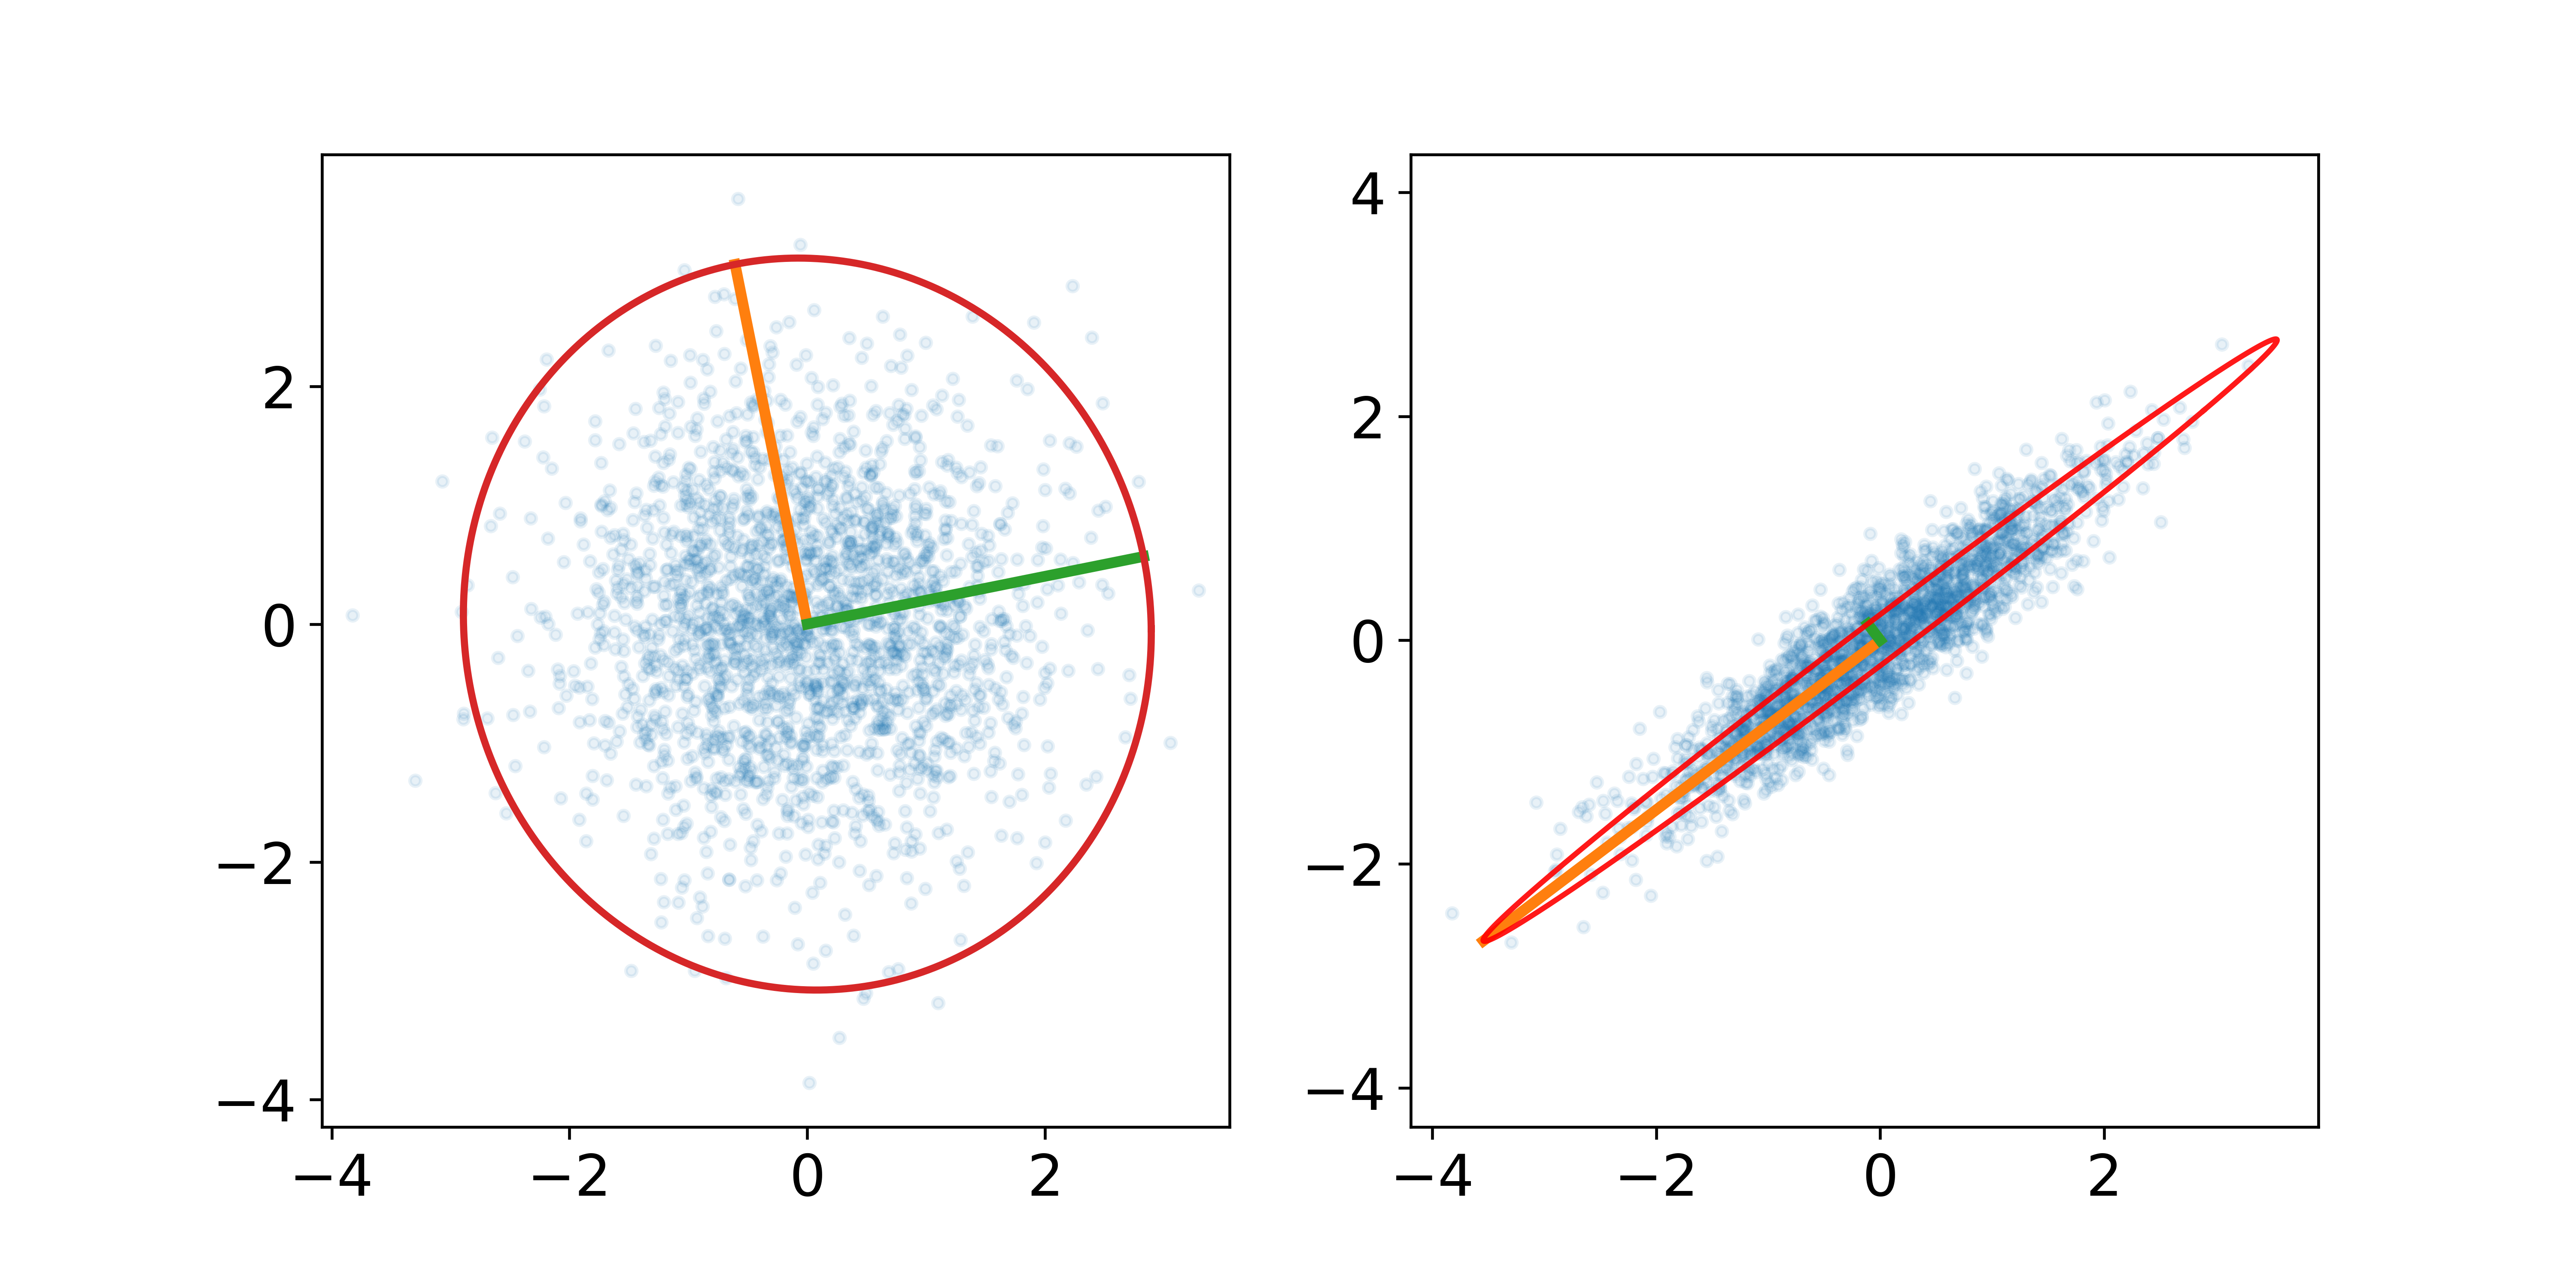
\includegraphics[width = 0.5\textwidth]{pca.png}
% \end{figure}
% \end{frame}

\end{document}